\section{Datasets}
\label{sec:datasets}

\subsection{Nursing}

Table \ref{tab:datasets} and Figure \ref{fig:coverage} 
give a breakdown of the size and content of the Nursing dataset.

\begin{table}[!h]
    \centering 
    \caption{Nursing dataset: total and unique row counts for schemas, test sets, and example sets.
    % for Hospitals A--D.
    }
    \label{tab:datasets}
    \begin{tabular}{crrrrr}
        \toprule
        \textbf{Hospital} & \textbf{Sch.} & \multicolumn{2}{c}{\textbf{Test}} & \multicolumn{2}{c}{\textbf{Examples}} \\
        \cmidrule(lr){3-4}
        \cmidrule(lr){5-6}
        & & tot. & un. & tot. & un. \\
        \midrule 
        A & 1064 & 739 & 133 & 1816 & 149 \\
        B & 1118 & 308 & 108 & 881 & 210 \\
        C & 601 & 741 & 169 & 2176 & 170 \\ 
        D & 1261 & 551 & 166 & 1424 & 192 \\
        \bottomrule
    \end{tabular}
\end{table}

\begin{figure}[h]
    \centering
    % \hfill
    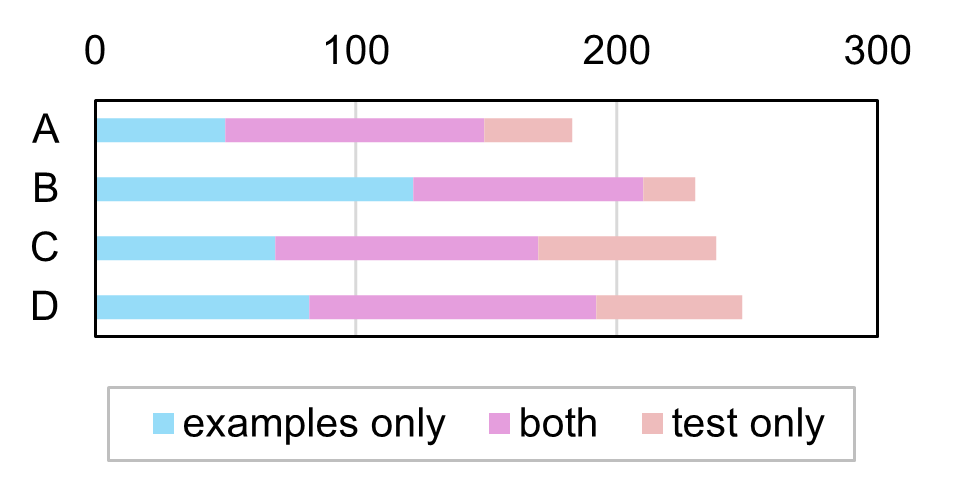
\includegraphics[width=.9\linewidth]{img/coverage.png}
    \captionof{figure}{Counts of unique rows that appear in each Hospital's test set, example set, or both.}
    \label{fig:coverage}
\end{figure}

\subsection{Amazon}
\label{sec:datasets-amazon}

% \textbf{Amazon.}~~ For variety in domain, we also evaluate our method a subset of the publicly available sample of the Bright Data Amazon Products dataset \cite{brightdata2025}. 
% This dataset contains metadata from 1000 scraped Amazon product webpages, including various prose features and a set of annotated key-value pairs for each product. We randomly sample a maximum of two products per annotated ``department'' key, resulting in a total of 48 products in our subset. We prepare a transcript for each by concatenating the product title, description, top review, product dimensions, weight, manufacturer, and bullet point prose features into a string. We also manually review the key-value pairs (discarding ``department'') to ensure they can be substantiated by the transcript content. This test set contains 804 annotated key-value pairs and 554 unique keys. 

% Collecting and cleaning all keys, values, and product categories (groups) over the full 1000 products, we assemble a schema $S_{\mathrm{Am}}$, which contains 1906 rows and 902 groups and uses four row types: Single, Multi, Numeric, and Weight. All annotated rows in the test set are present in $S_{\mathrm{Am}}$.
The Amazon dataset used in this work (the ``Subset'') is a subset of the publicly available sample of the Bright Data Amazon Products dataset \cite{brightdata2025} (the ``Public Sample''). While the Public Sample is clearly labeled as publicly downloadable, it does not come with a named license. Therefore, out of an abundance of caution and wish to abide by any existing copyright restrictions, we do not release our Subset derived from the Public Sample. We instead describe our process for internally creating the Subset here.


The Public Sample consists of scraped data from 1000 Amazon product webpages, including various prose features and a set of annotated key-value pairs for each product. To transform this data into a schema and test set suitable for structured information extraction, we follow the steps outlined below.

\textbf{Schema preparation.}~In the Public Sample, each product has a list of annotated groups $G = \{g_0, ..., g_n\}$ and a set of annotated key-value pairs. We form the schema $S_{\mathrm{Am}}$ by creating a distinct row for each unique $g_0$--key combination, taken from across all 1000 products. Possible values for each of these rows are collected from every instance of the $g_0$--key combination in the Public Sample. Each row's categories $C$ are the set of all groups from the products where the row's $g_0$--key combination is present.

After assembling possible values for every row in this way, closer attention is needed. We discard all rows with metadata not in English. For rows with values containing commas, semicolons, or other obviously delimited lists of choices, we split each delimited string into its own possible value and schematize the row as a Multi row. Rows that, on manual inspection, indicate numeric values or weights are schematized as Numeric or Weight rows, respectively. All remaining rows are schematized as Single rows.

Single rows for which the above process yielded only one possible option are either ``hydrated'' when reasonably completable (\textit{e.g.}, a Single row only containing a ``yes'' option is also supplied a ``no'' option) or discarded.

\textbf{Test set preparation.}~We randomly sample a maximum of two products per annotated ``department'' key, resulting in a total of 48 products in the Subset. For each of these products, we prepare a transcript by concatenating the product title, description, top review, product dimensions, weight, manufacturer, and bullet point prose features into a single string. 

We also manually review the annotated key-value pairs (excluding ``department'') to ensure they can be substantiated by the transcript content. Key-value pairs that cannot be reasonably inferred from the transcript, such as serial numbers or model names that are never mentioned, are discarded from the annotations. When an option from the schema is clearly available and applicable to the transcript, we add it to the annotations. For example, if the transcript mentions a product is ``red and blue,'' and there exist ``red'' and ``blue'' Multi options in the appropriate schema row, but the original annotated value was ``red'' alone, we add ``blue'' to the values for that annotated key-value pair. Annotations that are plainly inconsistent with the transcript are corrected. For example, if the transcript mentions a quantity of ``3'' and the original annotated value was ``2,'' we correct the annotation to ``3.'' We also remove any duplicate key-value pairs from the annotations.
